\documentclass{article}
\usepackage{graphicx}
\usepackage{fontspec}
\setmainfont{Microsoft YaHei}
\usepackage{geometry}
\setlength{\parindent}{0pt}
\usepackage{ctex}
\usepackage{algorithm}  
\usepackage{algorithmicx}  
\usepackage{algpseudocode}  
\usepackage{amsmath}  
\title{Database HW6}
\author{王嵘晟 \quad PB1711614}
\date{}
\begin{document}
	\maketitle
	\section*{1.}
	\subsection*{(1).}
	首先,插入36: \\
	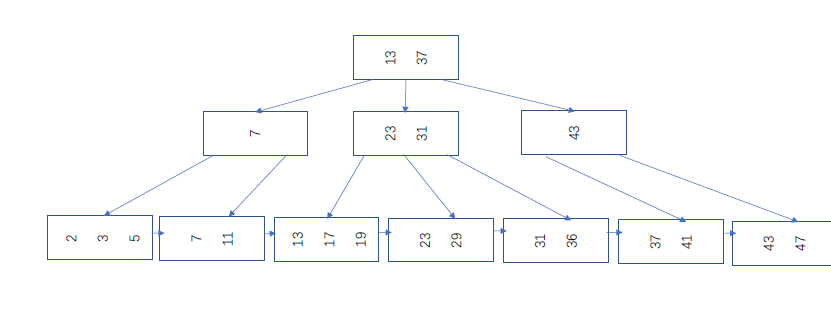
\includegraphics[scale=0.48]{2.png}\\
	插入18: \\
	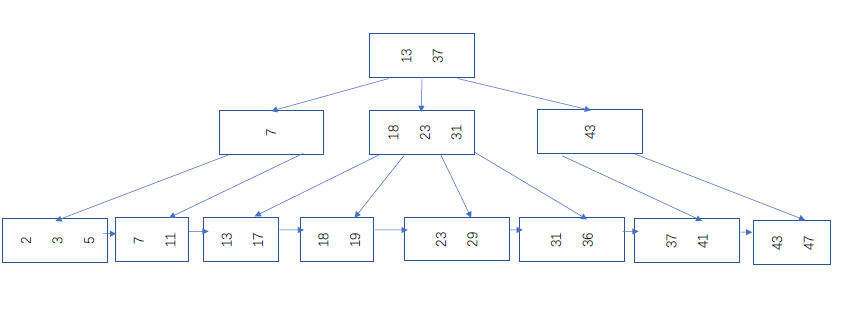
\includegraphics[scale=0.48]{3.png}\\
	插入40: \\
	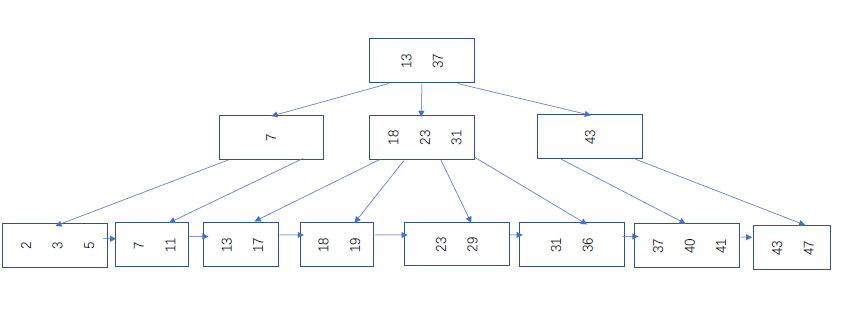
\includegraphics[scale=0.48]{4.png}\\
	\subsection*{(2).}
	首先,删除43: \\
	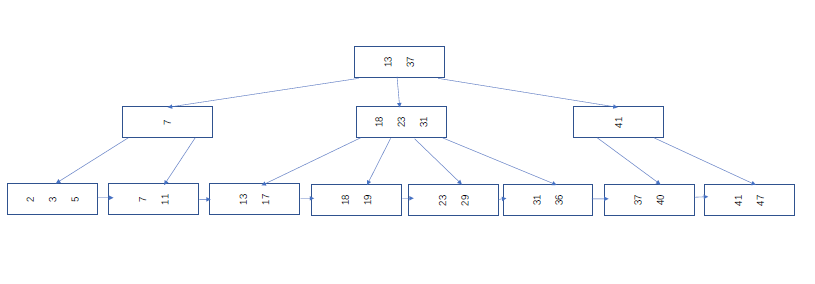
\includegraphics[scale=0.48]{5.png}\\
	删除13: \\
	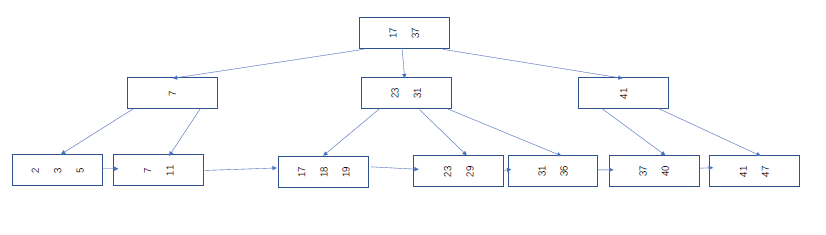
\includegraphics[scale=0.48]{6.png}\\
	删除7: \\
	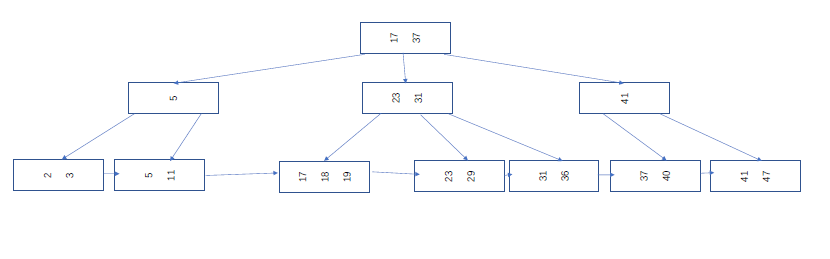
\includegraphics[scale=0.48]{7.png}\\
	\section*{2.}
	\subsection*{(1).}
	全部插入完成后可拓展散列表简图如下: \\
	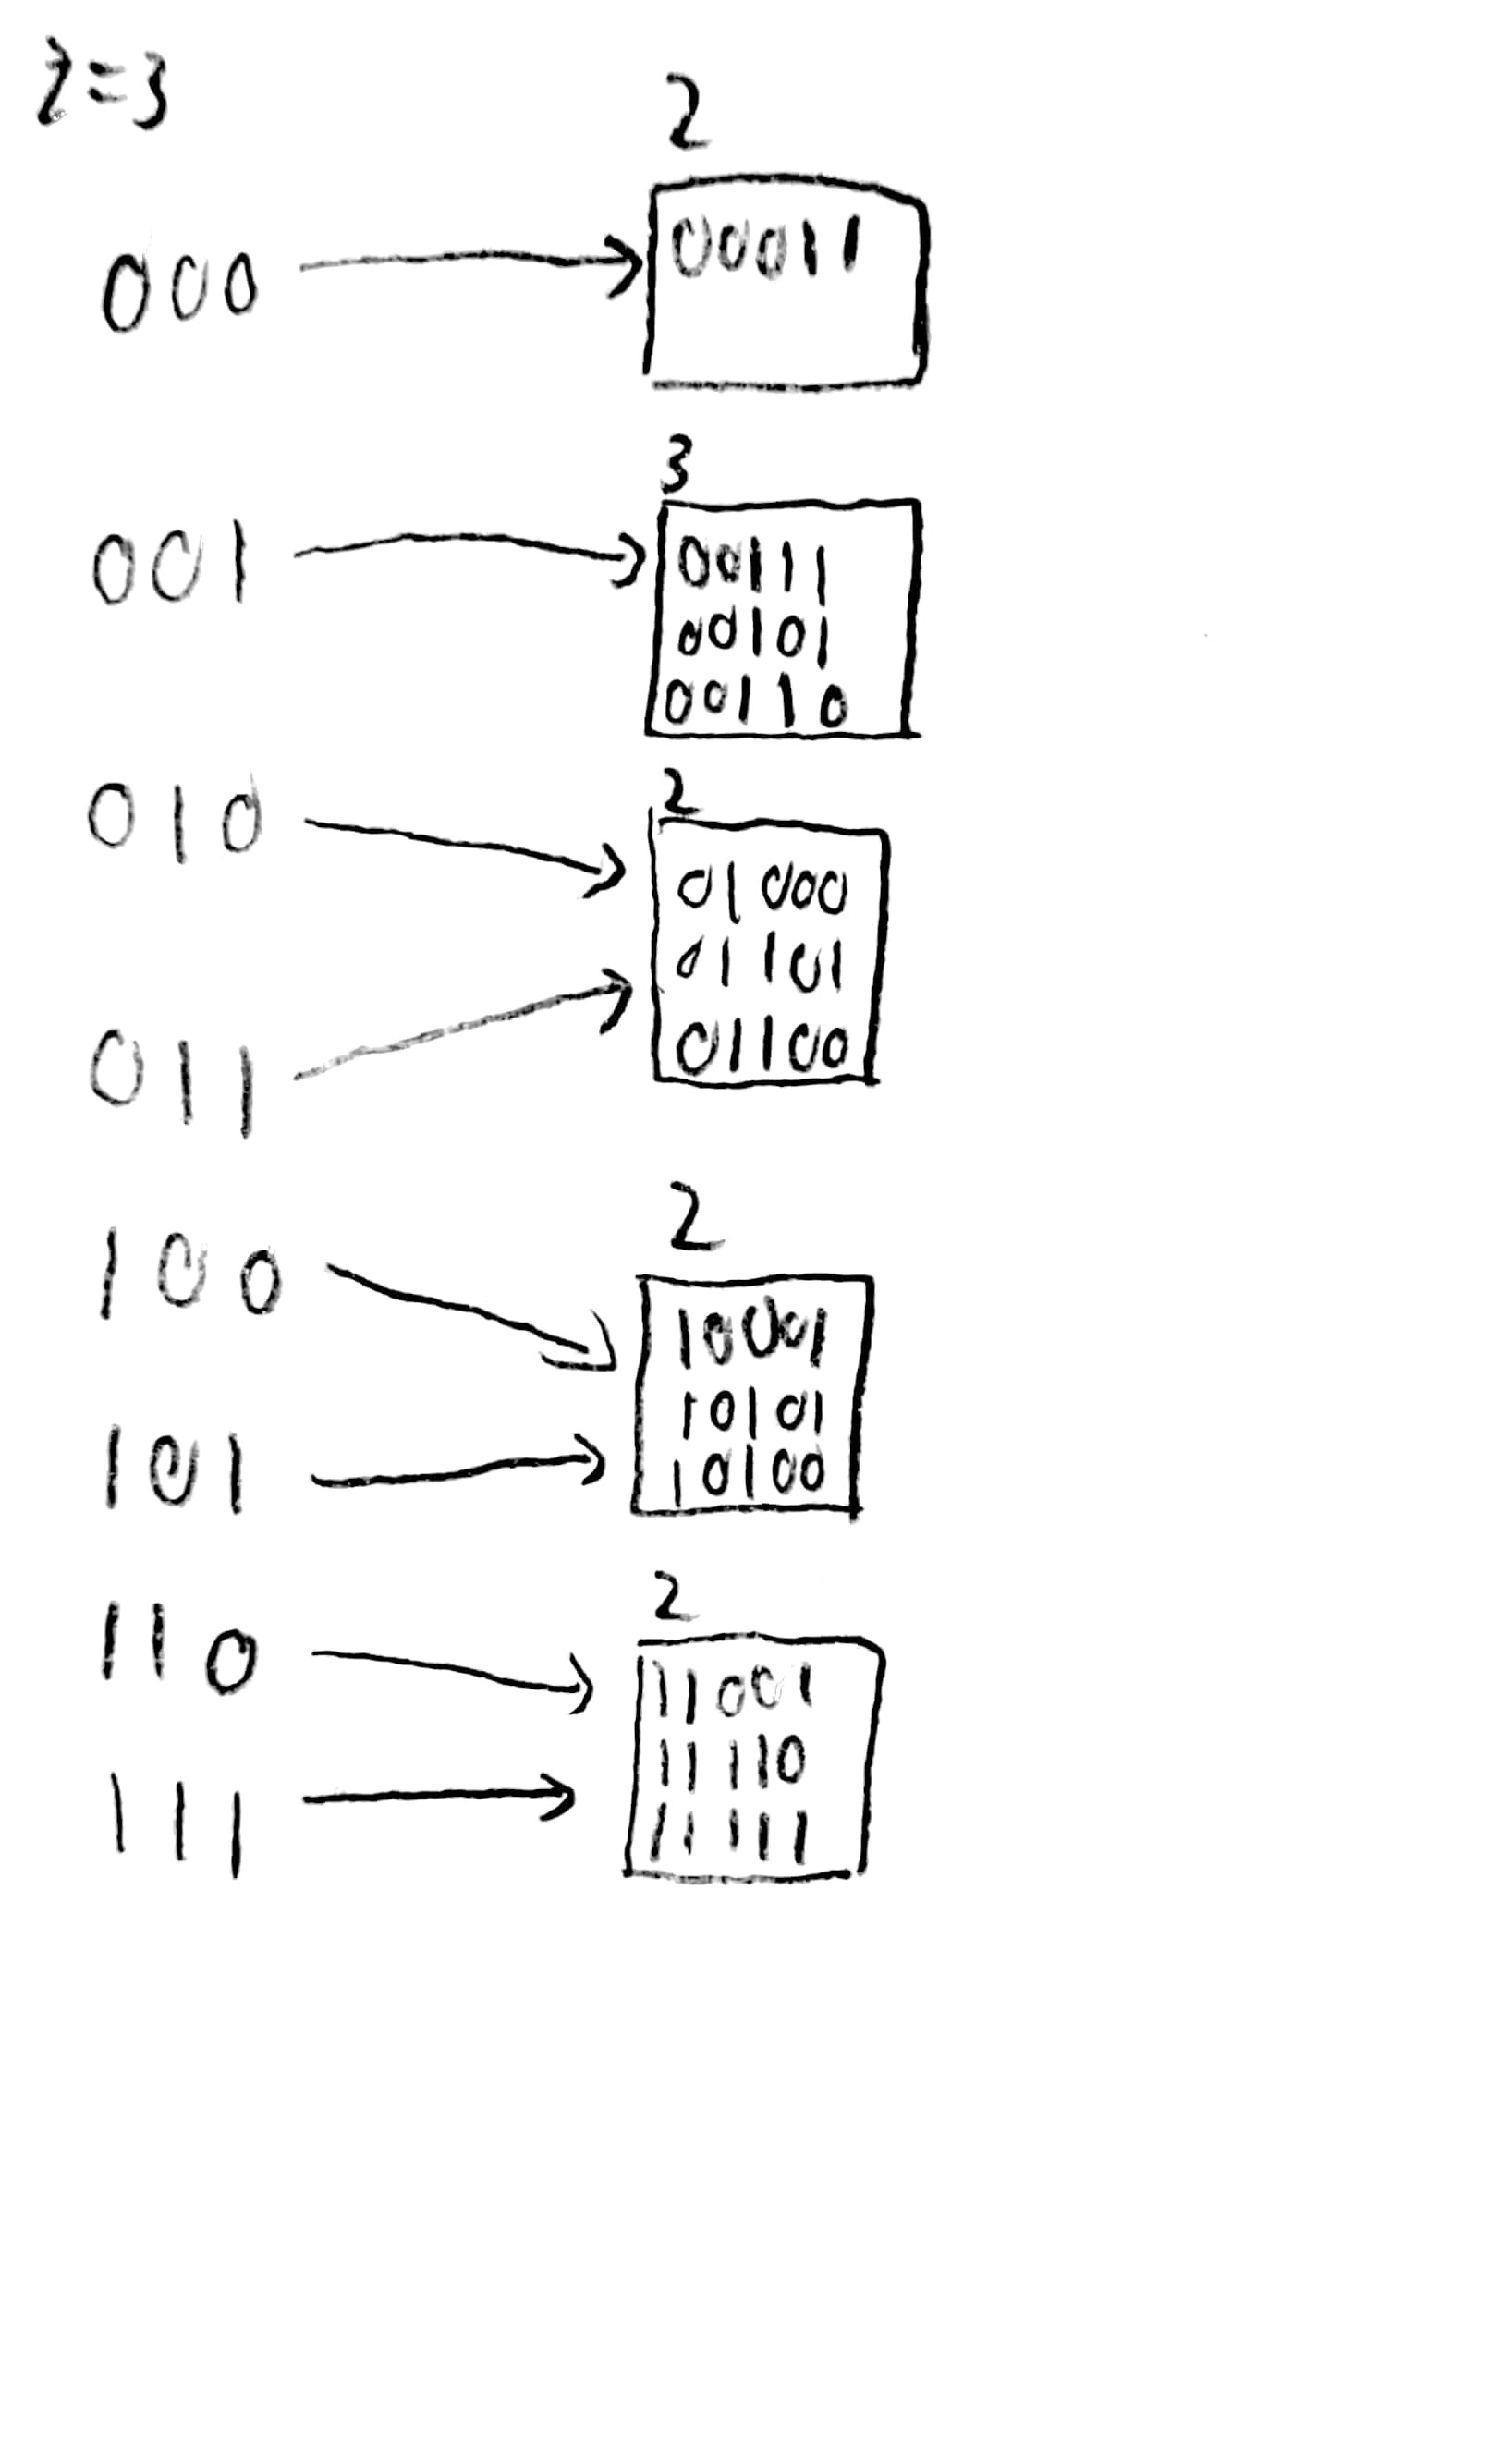
\includegraphics[scale=0.15]{8.jpg}\\
	所以共有5个桶,和E键值在同一个桶里的是10001,\ 10100,\ 10101
	\subsection*{(2).}
	由于空间利用率为$80\%$,所以$\frac{r}{n}<2.4$时不需要增加新桶。\\
	全部插入完成后的线性散列表简图如下: \\
	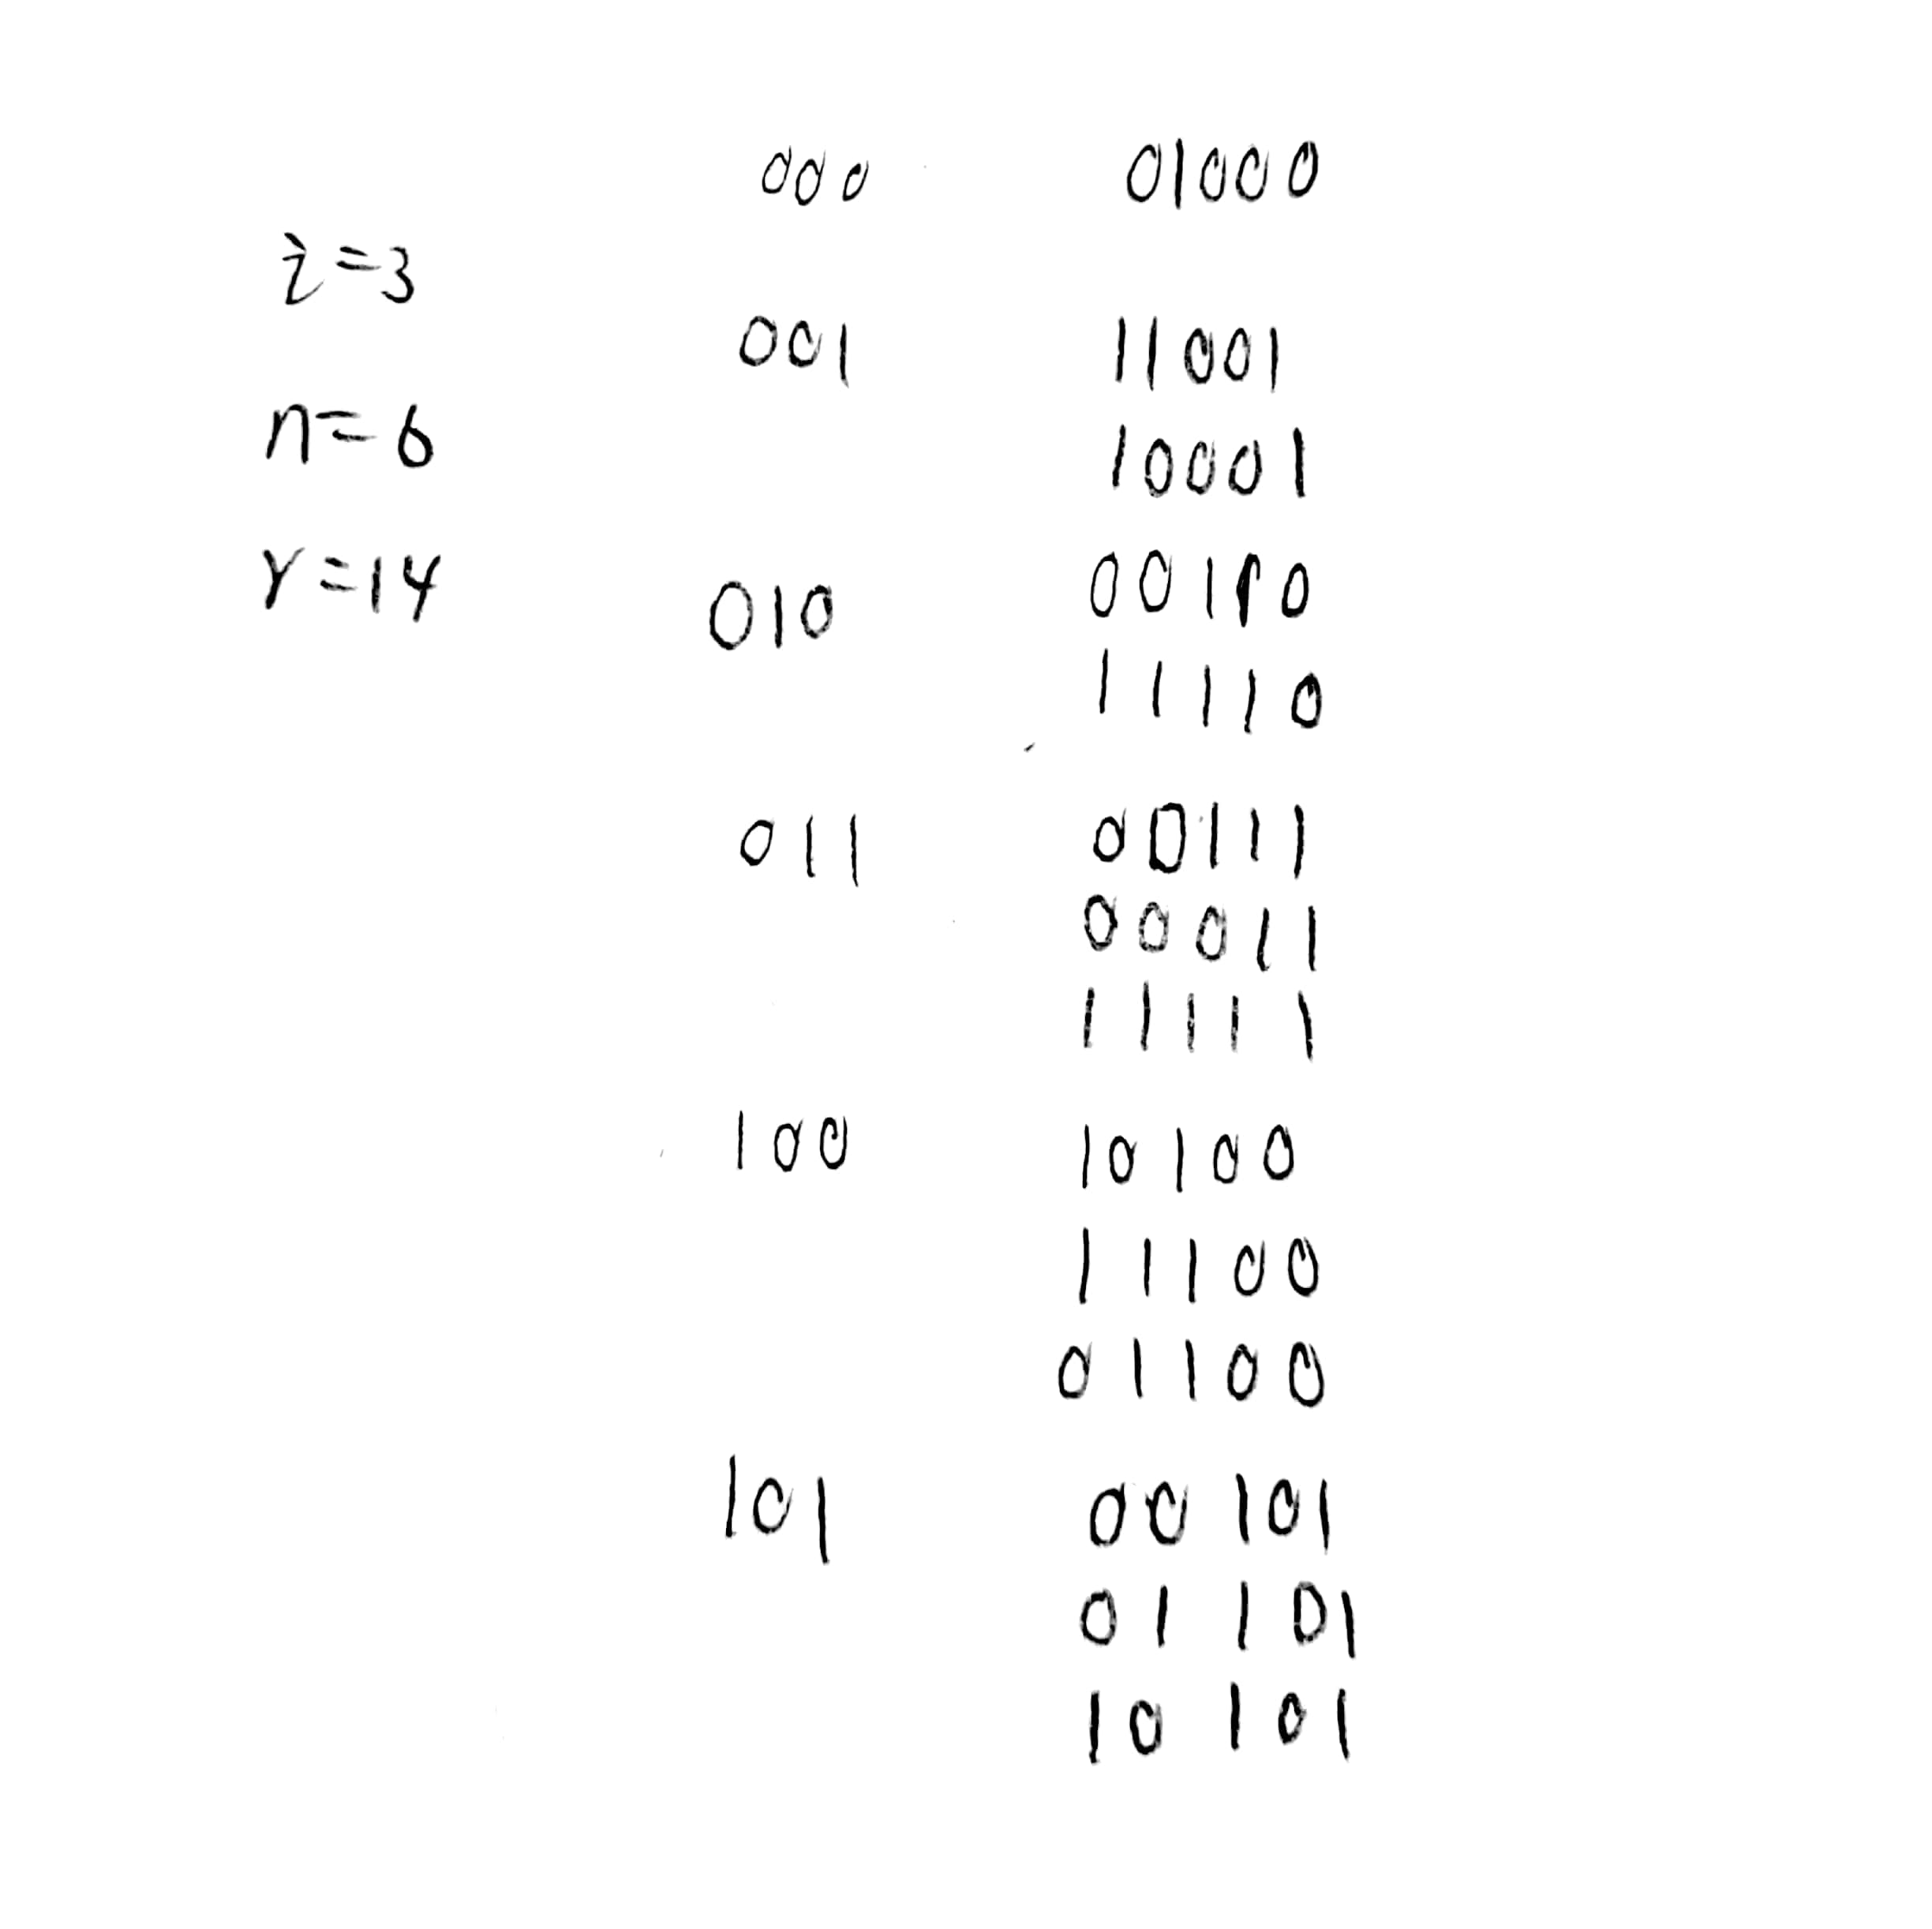
\includegraphics[scale=0.15]{9.jpg}\\
	可见一共有6个桶,和B键值在同一个桶中有00111,\ 00011,\ 11111
\end{document}